% general format definition
\documentclass[a4paper, 11pt]{article}
\usepackage[margin=.9in]{geometry}
\usepackage[utf8]{inputenc}
\usepackage[T1]{fontenc}
\usepackage[english]{babel}

% extra packages
\usepackage{hyperref}
\usepackage{listings}
\usepackage{color}
\usepackage{amsmath}
\usepackage{amsfonts}
\usepackage{amsthm}
\usepackage{mathtools}
\usepackage{microtype}
\usepackage{stmaryrd}
\usepackage{tikz}
\usetikzlibrary{arrows,automata,positioning}


% special math symbols
\newcommand{\R}{\ensuremath{\mathbb{R}}}
\newcommand{\N}{\ensuremath{\mathbb{N}}}
\newcommand{\Z}{\ensuremath{\mathbb{Z}}}
\newcommand{\Q}{\ensuremath{\mathbb{Q}}}

% Syntax highlighting
\definecolor{commentsColor}{rgb}{0.497495, 0.497587, 0.497464}
\definecolor{keywordsColor}{rgb}{0.000000, 0.000000, 0.635294}
\definecolor{stringColor}{rgb}{0.558215, 0.000000, 0.135316}
\lstset{
  backgroundcolor=\color{white},                        % choose the background color; you must add \usepackage{color} or \usepackage{xcolor}
  basicstyle=\footnotesize,                             % the size of the fonts that are used for the code
  breakatwhitespace=false,                              % sets if automatic breaks should only happen at whitespace
  breaklines=true,                                      % sets automatic line breaking
  captionpos=b,                                         % sets the caption-position to bottom
  commentstyle=\color{commentsColor}\textit,            % comment style
  deletekeywords={},                                    % if you want to delete keywords from the given language
  escapeinside={\%*}{*)},                               % if you want to add LaTeX within your code
  extendedchars=true,                                   % lets you use non-ASCII characters; for 8-bits encodings only, does not work with UTF-8
  frame=tb,	                   	                        % adds a frame around the code
  keepspaces=true,                                      % keeps spaces in text, useful for keeping indentation of code (possibly needs columns=flexible)
  keywordstyle=\color{keywordsColor}\bfseries,          % keyword style
  otherkeywords={True,False,true,false,null,None,NULL}, % if you want to add more keywords to the set
  numbers=left,                                         % where to put the line-numbers; possible values are (none, left, right)
  numbersep=5pt,                                        % how far the line-numbers are from the code
  numberstyle=\tiny\color{commentsColor},               % the style that is used for the line-numbers
  rulecolor=\color{black},                              % if not set, the frame-color may be changed on line-breaks within not-black text (e.g. comments (green here))
  showspaces=false,                                     % show spaces everywhere adding particular underscores; it overrides 'showstringspaces'
  showstringspaces=false,                               % underline spaces within strings only
  showtabs=false,                                       % show tabs within strings adding particular underscores
  stepnumber=1,                                         % the step between two line-numbers. If it's 1, each line will be numbered
  stringstyle=\color{stringColor},                      % string literal style
  tabsize=2,	                                          % sets default tabsize to 2 spaces
  title=\lstname,                                       % show the filename of files included with \lstinputlisting; also try caption instead of title
  columns=fixed,                                        % Using fixed column width (for e.g. nice alignment)
}

\author{Emma van Emelen}
\title{FoSAP Lecture Notes}
\begin{document}
    % titlepage
    \maketitle
    \newpage

    % contents
    \tableofcontents
    \newpage

    % section 1
    \section{Introduction}
    Look at the Following problem:\\
    \vtop{
      \texttt{Input: a string `w` consisting of 0s and 1s\\
              Examples: {\color{red}0101}, {\color{green}1001}, {\color{red}00110}, {\color{green} 0101010}\\
              Question: Are these requirements fullfilled?}
      \begin{itemize}
        \renewcommand\labelitemi{$\rightarrow$}
        \item 11 is not a sub-word
        \item \texttt{w} is divisible by 3 in binary
      \end{itemize}
    }
    \subsection{A Possible Solution (featuring cryptic C code)}
    \begin{lstlisting}[language=C]
int F[] = { 1, 0, 0, 0, 1, 0, 0 };
int delta[][2] = {{ 0, 1 },{ 3, 6 },{ 3, 4 },{ 2, 5 },{ 0, 6 },{ 2, 6 },{ 6, 6 }};

int three_not_11(char *w)
{
    int q = 0;
    while( *w ) q = delta[ q ][ *w++ - '0' ];
    return F[q];
}
    \end{lstlisting}
 
    \subsection{Finite Automation}
    The above C code essentially simulates the following finite automaton:
    \begin{figure}[h]
      \centering
      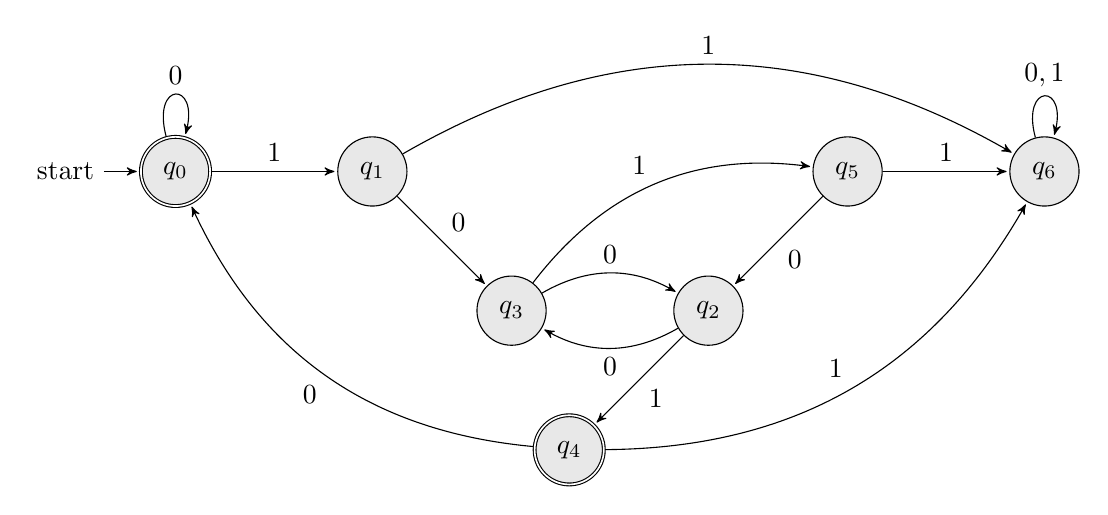
\begin{tikzpicture}[->,>=stealth',shorten >=1pt,auto,node distance=2.5cm,
            scale = 1,transform shape]
            \tikzstyle{every state}=[fill={rgb:black,1;white,10}]
            \node[state,initial, accepting] (q_0) {$q_0$};
            \node[state] (q_1) [right of=q_0] {$q_1$};
            \node[state] (q_3) [below right of=q_1] {$q_3$};
            \node[state] (q_2) [right of=q_3] {$q_2$};
            \node[state, accepting] (q_4) [below left of=q_2] {$q_4$};
            \node[state] (q_5) [above right of=q_2] {$q_5$};
            \node[state] (q_6) [right of=q_5] {$q_6$};

            \path[->]
                % from q_0
                (q_0) edge [loop above] node {$0$} (q_0)
                (q_0) edge []           node {$1$} (q_1)

                % from q_1
                (q_1) edge []           node {$0$} (q_3)
                (q_1) edge [bend left]  node {$1$} (q_6)

                % from q_3
                (q_3) edge [bend left]  node {$0$} (q_2)
                (q_3) edge [bend left]  node {$1$} (q_5)

                % from 
                (q_2) edge [bend left]  node {$0$} (q_3)
                (q_2) edge []           node {$1$} (q_4)

                (q_4) edge [bend left]  node {$0$} (q_0)
                (q_4) edge [bend right] node {$1$} (q_6)

                (q_5) edge []           node {$0$} (q_2)
                (q_5) edge []           node {$1$} (q_6)

                (q_6) edge [loop above] node {$0,1$} (q_6)
                ; 
      \end{tikzpicture}
      \caption{The Finite Automaton}
    \end{figure}
    \\This automaton works in the following way:
    \begin{itemize}
      \item[$q_0$ -] the inital state, as well as an accepting state, we return true, if we end here
      \item[$q_4$ -] an accepting state, we return true, if we land here 
      \item[$q_6$ -] the default false state, if we have \texttt{11} as subword
      \item[$other$ -] if we end on any other state, we also return false, because it isn't divisible by 3   
    \end{itemize}
    \newpage

    \section{Words and Languages}
    \subsection{What is a word and what is a language?}
    An informal answer to the question could be, that a word $w$ is a concatenation of symbols $s$ in a specified alphabet $\Sigma$.
    A language $L$ would then be a set of words defined by a pattern, like $\{a^{n^{2}}|n \geq 0 \} = \{\epsilon, a, aaaa, aaaaaaaa, \dots\}$.
    \\
    Words have a natural and intuitive mathematical structure. We can concatenate words, split a word, and parse sentences naturally. 
    We can also get a section of the word and remove parts to get a new word.
    \begin{itemize}
      \centering
      \item[Flughafen $\rightarrow$] Flug \& Hafen
      \item[Baumhaus $\rightarrow$] Baum \& Haus  
    \end{itemize}
    In the case of natural language, if it uses latin characters, the alphabet and language is easily defined:

    \begin{align}
            L = & \mbox{ } \{s^* | s\in \Sigma\} = \{a, a, they, them, you, ich, er, sie, \dots\}\\
       \Sigma = &\mbox{ }  \{a,b,c,\dots,x,y,z,A,B,C,\dots,X,Y,Z\}
    \end{align}
    As we can see here, the alphabet $\Sigma$ is just every uppercase and lowercase latin character and our language $L$ is
    no more than a set of words that have one or more character $s\in\Sigma$.

    \subsection{The Formal Definition}
    \begin{itemize}
      \item A semigroup $(H, \circ)$ consists of a set $H$ and an associative relation $\circ:H\times H \rightarrow H$
      \item A \emph{monoid} is a semigroup with a neutral element
      \item Let $(M, \circ)$ be a monoid and $E \subseteq M$\\
            $E$ is a generating system of $(M, \circ)$ , if every $m\in M$ can be represented as $m=e_1\circ\dots e_n$ with $e_i \in E$.
            A neutral element $e$ is left and right neutral. $\forall x : e\circ x = x\circ e = x$.
    \end{itemize}
    A great example, using what we already established, would be to define the Alphabet $\Sigma$ as the generating system of our monoid 
    $(L, \circ)$ where $\circ$ is sefined as concatenation.

\end{document}